\chapter{Introduction, Problems and Goals}

\section{Introduction to ONOS}

\subsection{Computer networks}

With the term "computer network" we refer to a network of interconnected digital devices sharing data. This is maybe the easiest definition we can find, but we are missing quite a lot of useful information. For example, we can add that it's not important the types of devices we use: using the appropriate tools and technologies we can put in the same network different devices having different (even opposite) characteristics: huge high-performant workstations, laptops, little smart devices, smart fridges and so on. These devices can use different methods to communicate, like wires (several types and categories e.g. coaxial cable, twisted pair, optical fiber...) and wireless radio-frequency methods. There are three main types of 'architectures': client-server, peer to peer and a mixed solution. The most used is the first one: a client requests services to a server that has the goal of serving the clients, simple as that. We can also add we have to use communication protocols to effectively share data; each device or node in the network must know how to receive a message, how to read and interpret the data, and how to reply to all or a specific recipient node. Over the years research scientists and universities all across the earth developed thousand of protocols to have a reliable and effective connection. Some of the most famous ones are TCP, UDP, IP, HTTP, and DNS. These protocols are used in the TCP/IP stack (graphically shown in Figure 1.1) we use every day accessing Internet. 

\begin{wrapfigure}[17]{r}{0.55\textwidth}
\caption{TCP/IP protocols suite (docs.oracle.com)}
\label{fig:tcpipstack}
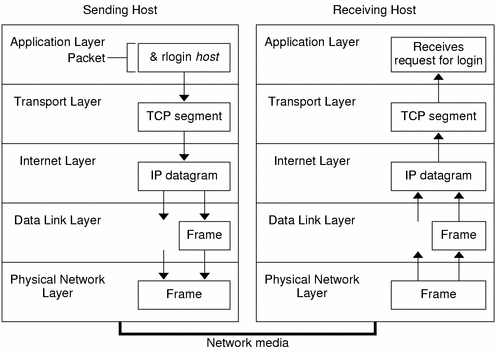
\includegraphics[width=0.55\textwidth]{resources/Chapter-1/tcpipstack.jpeg}
\end{wrapfigure}

The idea behind this stack is really simple: there are five layers (physical, data, network, transport, and application) and each one provides services for the upper layer. The figure shows a usage example of the stack: an application creates its packet and it sends that 'down' to the transport layer. This layer will add an header containing information useful for the transport layer of the receiving host. This step is repeated until the final packet is created, and finally, that packet can be sent over the network. The host receiving a packet will do the same steps but in the opposite direction, removing headers until it gets the final application layer data. It has many advantages: (a) It's an open protocol suite. No one owns that and can be used by anyone. (b) It's a scalable architecture. Nodes can be added to the network without disrupting the services. (c) It's modular by design. This means we can completely change protocol at a certain level, but the upper layer will remain unchanged. Another big advantage of this suite is the fact that not all the devices in the network must implement or be aware of all the layers in the stack, but only the ones they directly use. For example a router, the device routing the packets in the network, must know only about the first three layers and can ignore the two upper layers (transport and application) as it doesn't provide services using those layers. Of course, this is not the only existing protocols suite, but for sure is the most used one. It's crucial to notice that the Internet is important because is the biggest and most famous computer network, but even the simplest networks follow the same rules (e.g. two computers connected by a cable).

\subsection{Software Defined Networking}

A particular type of computer network is a Software Defined Network (SDN). In traditional networks, we have distributed devices (they can be emulated also in the same machine, but generally they are physically located in different places) implementing protocols and technologies they need to make the network works as intended. In order to have a working network each device must know some information to deliver packets to other nodes in the same network or other subnetworks. This requires nodes in the network actively or passively gather that information, for example we can talk about routing. Let's say we have several end hosts in the network connected using routers. Those routers only know they have to use a specific routing protocol (e.g. OSPF) to make those hosts communicate effectively. Each router must fill its routing table in order to understand for a packet having specific characteristics which route has to be chosen. This means each device in the network has a local view of the whole network: a router only knows about its neighbors and how to deliver a packet to the next device. Doing so can be highly inefficient, this is one of the main reasons why Software Defined Networking has been invented.
 
Feamster et al. defines Software Defined Networking using these words \cite{sdn-definition}:
\begin{quoting}[font=itshape, begintext={"}, endtext={"}]
First, an SDN separates the control plane (which decides how to handle the traffic) from the data plane (which forwards traffic according to decisions that the control plane makes). Second, an SDN consolidates the control plane, so that a single software control program controls multiple data-plane elements. The SDN control plane exercises direct control over the state in the network’s data-plane elements (i.e., routers, switches, and other middleboxes) via a well-defined Application Programming Interface (API).
\end{quoting}

The main idea behind Software Defined Networking is to separate the concept of routing and forwarding. Routing is the act of determining which route has to be chosen for a packet having specific characteristics (source and destination addresses/networks or protocol-specific information), while forwarding is the concrete action of copying the entire packet from the ingress point to the egress point. A Software Defined Network is composed of multiple logical components: the Data Plane is the layer comprising the end hosts and the physical devices (e.g. switches); the Control Plane is the layer taking care of the routing process (let's say the brain, where the computation is centralized) and the Application Plane, where the software controlling and configuring the control plane is placed. As stated above, one main limitation of traditional networking is the limited view of the whole network, and so limited monitoring too. We are going to see some improvements brought by Software Defined Networks and main reasons of its usage.

During the latest years we've seen some changes in how people access and use the Internet. When a user requests a resource it's increasingly frequent to generate many requests in the back end: if we think of a web page it's not anymore a linear sequence of requests, but a compound of microservices, APIs, asynchronous and internal calls. Moreover, we have many devices connected sending data over the networks (personal devices like laptops, smartphones and tablets, but also smart devices and appliances). Another big change is the mad run to the cloud, both private, public and mixed one. Enterprises want the elasticity and scalability of cloud services to satisfy the needs of their customers. This means they should embrace powerful monitoring technologies, security by design and effective resource provisioning. The last change we faced and still we are facing in these years is the rise of what we call "Big data". First of all, we need big datasets for data mining and to accurately train machine learning models powering search recommendations, automation, pattern recognition and many others tasks in popular products. Secondly, as the number of people having access to the Internet is constantly increasing, a huge load of data is uploaded to datacenters every day; so we can say is like a fire that feeds itself.

All these changes led to the idea of having a centralized core component controlling and having a clear view of the network. This better visibility provides greater scalability, effective automation and more efficient network management.

Obviously it's not only about improvements, there are drawbacks too. Centralization could be very effective in management but it is very risky when it comes to security. This concept is named "single point of failure", it means that if some subcomponent in the central core is vulnerable the whole core could be at risk. The damage of this weakness can be reduced by applying the concepts of Compartmentalization and Defense in depth. The first one refers to the act of creating multiple compartments and separating the sub-services into containerized boxes checking the accesses from one to the other; this reduces the risk of one subcomponent affecting the others. The second one instead means applying multiple layers of security to avoid that a single security check bypass discovered by an attacker can disrupt the services.


\subsection{The Open Network Operating System} 

The Open Networking Foundation (abbreviated ONF) is a non-profit organization founded in 2011 to promote SDN-related technologies and standards. It uses an open source model (that's why Open is in the name) and the products involve wireless and telecommunications networks, datacenters and other networking areas. At the time of writing the foundation includes many famous companies and vendors, ranging from networking-equipment, semiconductor, computer and software companies, telecommunication service providers and datacenter operators. Among these members we can see Google, Microsoft, AT\&T, Cisco, Intel, NVIDIA and many others. In 2011 the foundation started to promote control and forwarding planes decoupling introducing and supporting SDN concepts; the next year they open sourced Openflow that is the first protocol standard to enable remote network controllers managing the nodes in the data plane. In 2014 the foundation 
 released the first open source version of the Open Network Operating System (ONOS), the leading open source SDN Controller. Three years later they released CORD, an edge-cloud solution for telecommunication and cable operators \cite{opennetworking-org}.

ONOS development started in 2014, the source code is available on GitHub platform and at the time of writing it counts more than 260 individual contributors \cite{github-onos}. It's mainly written using Java, but many technologies and programming languages are used for the whole project, like Python, Jinja, JavaScript and Typescript, OSGi, Bazel files, Swagger and many more. The term SDN Controller can be ambiguous since it's a real operating system and like any operating system it uses a kernel and installable applications. ONOS uses as "base layer" Apache Karaf which is a polymorphic application container. It means it is a technology to deploy together various services and components in the same environment giving them the ability to communicate and share resources. It uses the "run anywhere" concept, meaning that it can be used with bare hardware using Java, Docker images or cloud instances. The Apache Foundation in the official documentation states that among many features it supports hot deployment, dynamic configuration, advanced logging system and a UNIX-like console to interact with the runtime. Looking at the logical ONOS architecture (shown in figure 1.2), we can see many components:

\begin{itemize}
  \item \texttt{Applications}: The applications are OSGi bundles that can be activated and deactivated (both at system startup and at runtime using the Karaf console) providing and implementing services ranging from displaying network topologies in a web browser, integrating famous products in ONOS (like Kubernetes and Apache Kafka) to setting up flow rules for custom network traffic.
  \item \texttt{Northbound API}: Northbound APIs is the way applications and core component communicate. The applications can receive notifications and alerts from the Core, listen for events regarding specific topics, overwriting values in core sub-components (data stores and settings) and ask for additional resources.
  \item \texttt{Core}: The Core is the main component, hosting data stores and services for managing various subsystems like Devices, Link, Host and many others. We'll see later why it's distributed. 
  \item \texttt{Southbound API}: Southbound APIs is the way core component and network nodes in the data-plane communicate. The Core can receive notifications and alerts for the network, listen for events regarding specific topics and react to incoming data-plane messages.
  \item \texttt{Providers}: Providers are protocol-aware components for interacting with network devices. They can translate incoming data from the network to messages understandable by the Core. 
\end{itemize}

\begin{figure}[t]
\caption{ONOS architecture (opennetworking.org/onos/)}
\label{fig:onos-arch}
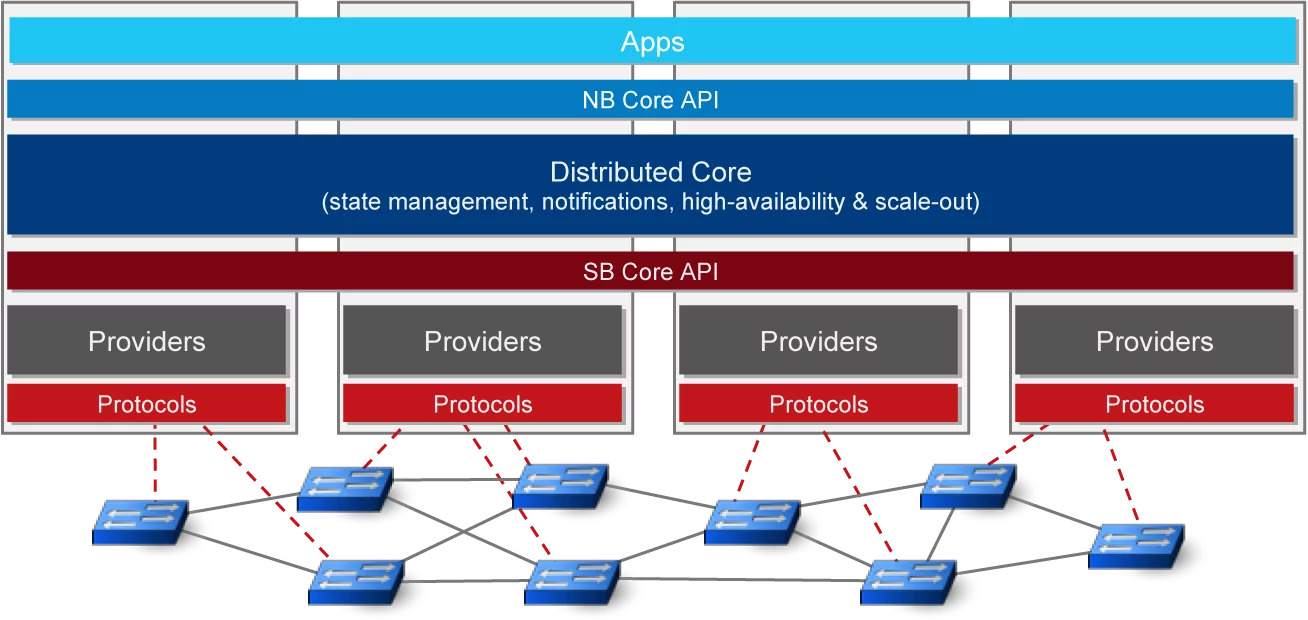
\includegraphics[width=1.0\textwidth]{resources/Chapter-1/onos-arch.jpg}
\centering
\end{figure}

In ONOS the term "service" is a vertical slice through the horizontal logical components of the figure 1.2. For example the Device service (or subsystem) is a vertical slice comprising applications, Northbound APIs, core components, Southbound APIs and Providers managing the devices in the network. The Software Defined Networking concept was presented talking also about the 'centralization' of the information, but in the figure we can read 'Distributed Core'. This is an important feature of ONOS: we can use multiple controllers in order to have a fault tolerant and highly available environment. Even if this feature is really powerful, during this research activity only single controller environments have been taken into account. 

As stated in the subsection title this is just a gentle introduction to ONOS, its components and their purposes, for a more detailed study of the ONOS architecture and internals go to Section 2.1 (ONOS internals).  

\clearpage

\section{Introduction to CAP attacks}

\subsection{Attacks targeting SDN}

Software Defined Networking enhances the visibility and monitoring of the whole network having aggregated data of all the network packets and information in a single place. Despite this improvement, there are security drawbacks too. This new concept of networking adds complexity and this introduces new vulnerability types that were not present in traditional networks. Scott-Hayward et al. did an amazing work in "SDN Security: A Survey" listing and classifying security issues for Software Defined Networks \cite{sdn-security-survey}.

\begin{table}[h]
\begin{tabular}{llllll}
\hline
\thead{Security Issue/Attack} & \thead{Application} & \thead{App-Ctl} & \thead{Control} & \thead{Ctl-Data} & \thead{Data} \\ \cline{1-6}
\hline

\makecell[l]{Unauthorized Access\\ (e.g. Unauthorized Controller Access \\and Unauthenticated Application)} & \multicolumn{1}{l}{x} & \multicolumn{1}{l}{x} & \multicolumn{1}{l}{x} & \multicolumn{1}{l}{x} & \multicolumn{1}{l}{x} \\ \cline{1-6}

\makecell[l]{Data Leakage\\(e.g. Flow Rule Discovery and\\ Forwarding Policy Discovery)} & \multicolumn{1}{l}{} & \multicolumn{1}{l}{} & \multicolumn{1}{l}{} & \multicolumn{1}{l}{} & \multicolumn{1}{l}{x} \\ \cline{1-6}

\makecell[l]{Data Modification\\(e.g. Flow Rule Modification)} & \multicolumn{1}{l}{} & \multicolumn{1}{l}{} & \multicolumn{1}{l}{x} & \multicolumn{1}{l}{x} & \multicolumn{1}{l}{x} \\ \cline{1-6}

\makecell[l]{Malicious Applications\\(e.g. Fraudulent Rule Insertion\\ and Controller Hijacking)} & \multicolumn{1}{l}{x} & \multicolumn{1}{l}{x} & \multicolumn{1}{l}{x} & \multicolumn{1}{l}{x} & \multicolumn{1}{l}{x} \\ \cline{1-6}

\makecell[l]{Denial of Service\\ (e.g. Controller-Switch Communication\\ Flood and Switch Flow Table Flooding)} & \multicolumn{1}{l}{} & \multicolumn{1}{l}{} & \multicolumn{1}{l}{x} & \multicolumn{1}{l}{x} & \multicolumn{1}{l}{x} \\ \cline{1-6} 

\makecell[l]{Configuration Issues\\(e.g. Lack of TLS Adoption \\ and Policy Enforcement)} & \multicolumn{1}{l}{x} & \multicolumn{1}{l}{x} & \multicolumn{1}{l}{x} & \multicolumn{1}{l}{x} & \multicolumn{1}{l}{x} \\ \cline{1-6} 
\end{tabular}
\end{table}

In the table above we can see the security issues categorized into six categories and marked with a cross which logical layers of Software defined networks are affected or targeted by these attacks. It's important to note that some of the categories are already present in traditional networks (like Data Leakage or Denial of Service), while certain classes are present only in Software defined networks. The most critical ones are the three classes affecting all the layers (Unauthorized Access, Malicious Applications and Configuration issues), but if we think about traditional networks, only Malicious application attacks are present only in Software defined networks. Some of the security issues are explained in the next pages, while certain ones are studied in a more detailed manner.

As we can see from the Software defined networks high-level overview described in subsection 1.1, these types of networks add complexity and have many components that need to communicate to make the networking effective and efficient. This detail introduces a new class of attacks called "Poisoning Attacks" that can put at serious risk many components of the network. Sattolo et al. published the paper "Classifying Poisoning Attacks in Software Defined Networking" with the aim of classifying these attacks using different metrics (by outcome, by layer and by requirements) \cite{class-poison-attacks}. A list of basic attacks with their brief description is presented below (basic means no active security mechanisms in place):

\begin{itemize}
  \item \texttt{Control Channel Hijacking}: The attacker reconfigures the targeted switches to use a different controller
  \item \texttt{Link Fabrication}: The controller thinks that between two devices there is a legitimate link, while in reality they are connected using a malicious host (can be performed using LLDP Packet Generation or LLDP Packet Relay) 
  \item \texttt{Host Location Channel Hijacking}: A malicious host to receive packets meant for another (can lead to data leakage and one-way denial of service)
  \item \texttt{Brain Racing}: Race condition in the source code of controller exploited by hosts 
  \item \texttt{Cross-App Poisoning}: Low privileged applications influences high-priviled applications taking some actions forbidden for the first type of applications. 
  \item \texttt{Teleportation}: Covert channel between a switch and another one (or even an host) undetected by the controller
\end{itemize}

It's important to repeat that vulnerabilities and security issues for traditional networks are still present here (e.g. ARP poisoning), but it's possible to leverage aggregated data to defeat or detect certain types of these attacks.

\subsection{ONOS security mechanisms}
Northbound and Southbound APIs are the main ways for the core component to communicate with applications and network components. However, as said before these are logical layers and nothing stops applications from having direct access to Southbound APIs or any other misuse of these technologies. Let's describe some security issues with the example used in the official documentation. Let's pick this scenario: a simple network, a single ONOS controller and two applications: the first one generates the DeviceDisconnected event (notification directed to the core component telling that a device has been disconnected) consistently modifying the network topology; the second one removes all the devices (layer 2 devices and end hosts) in the network.
\begin{wrapfigure}[17]{r}{0.55\textwidth}
\caption{Security-Mode ONOS}
\label{fig:secmode}
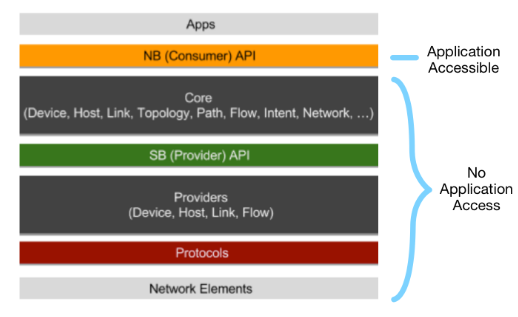
\includegraphics[width=0.55\textwidth]{resources/Chapter-1/sec-mode.png}
\end{wrapfigure}
These two applications could create problems related to the stability and reliability of the network. For example, if the environment uses the reactive forwarding application (org.onosproject.fwd) to add flow rules needed to correctly route the traffic, the choices made by this one could be unpredictable because the network could change in an inconsistent state due to the first two applications usage. One problem is clearly the fact that the first application generates the DeviceDisconnected events using the module called DeviceProviderService from the Southbound APIs. Applications should only use Northbound APIs, however since these are logical layers, they aren't directly connected in the conceptual drawings we use to explain the high-level architecture, but in reality nothing is blocking applications from importing and using those APIs (since they are public and can be used). The other problem is the fact that an application, even if it uses the Northbound APIs, is allowed to delete random devices (using one of the Admin Services), which is an important privilege that should be carefully granted only to selected few components in the environment. In order to prevent such types of APIs misuse, Security-Mode ONOS must be used. Using this mode it's possible to prevent applications from accessing sensitive ONOS tiers (only Northbound APIs allowed) and administrative actions; in particular three access methods are implemented: Bundle-level Role-based Access Control, Application-level Role-based Access Control and API-level Permission-based Access Control.
In order to use these access control mechanisms we need to specify a policy in the bundle specification file (needed to compile and install the application into ONOS). Here an example of a policy file for ONOS application:
\begin{lstlisting}[language=XML]
<feature name="onos-app-sdnip" version="1.0.0" description="SDN-IP peering application">
	<type> ONOS application </type>
	<role> non-admin </role>
	<uses-permission onos:name="onos.permission.INTENT_WRITE"/>
	<uses-permission onos:name="onos.permission.DEVICE_READ"/>
	<uses-permission onos:name="onos.permission.TOPOLOGY_EVENT"/>
	<uses-permission onos:name="onos.permission.PACKET_EVENT"/>
	<bundle>mvn:org.onosproject/onos-app-sdnip/1.0.0</bundle>
</feature>
\end{lstlisting}
In line 1 the feature field is used to specify some general information about the bundle. Line 2 specifies the bundle type and this is important to understand what the bundle is describing (could be a provider or a service), in this case being an ONOS application only the Northbound API access will be allowed. In line 3 the role field specifies if the bundle can access administrative services (can be 'admin' or 'non-admin'). From lines 4 to 7 the policy specifies which permissions the bundle is requesting access to; it's possible to define granular permissions for each application specifying the permission identifier (a complete list of all the permission identifiers can be found on the ONOS official documentation) \cite{secmode-perms}. Since this is a very important file for the security mechanism provided by ONOS, it's recommended to not only sign the jar file but also this policy file (e.g. using the JDK’s jarsigner). ONOS can also restrict the installation and deployment of applications from untrusted sources.

This is the order Security-Mode ONOS uses to check if a resource can be granted to a specific object, if all three checks pass the permission is granted, otherwise the action is blocked:
\begin{enumerate}
  \item\texttt{Bundle-level Role-based Access Control}: The "type" field in the bundle policy file is fetched, if the object is an ONOS application anything except the Northbound APIs is forbidden.
  \item\texttt{Application-level Role-based Access Control}: The "role" field in the bundle policy file is fetched, if the object role doesn't have administrator access some services are forbidden. 
  \item\texttt{API-level Permission-based Access Control}: The "uses permission" fields in the bundle policy file are fetched, then they are compared with the requested action to check if the object has all the required permissions. 
\end{enumerate}

Security-Mode ONOS and related suggested security mechanisms (like application and policy file signing) are crucial to secure the whole environment, however starting from ONOS version 2, the first mechanism is deprecated because it doesn't work with Apache Karaf version 4. 

The security mechanisms presented above are directly designed, implemented and provided by the ONOS developers community. Other mechanisms try to protect from specific attack types (such as the ones described in the previous section). We can see in the following table the defense mechanisms classification (by attack type) provided by Scott-Hayward et al.

\begin{table}[h]
\begin{tabular}{llllll}
\hline
\thead{Attack/Defense} & \thead{Host\\Location\\Hijacking} & \thead{Link\\Fabrication} & \thead{Cross-App\\Poisoning} & \thead{Control\\Channel\\Hijacking} \\ \cline{1-5}
\hline

\makecell[l]{TopoGuard\\Shutdown\\Checking} & \multicolumn{1}{l}{x} & \multicolumn{1}{l}{} & \multicolumn{1}{l}{} & \multicolumn{1}{l}{} \\ \cline{1-5}

\makecell[l]{TopoGuard\\HMAC} & \multicolumn{1}{l}{} & \multicolumn{1}{l}{x} & \multicolumn{1}{l}{} & \multicolumn{1}{l}{} \\ \cline{1-5}

\makecell[l]{Device\\Authentication} & \multicolumn{1}{l}{} & \multicolumn{1}{l}{} & \multicolumn{1}{l}{} & \multicolumn{1}{l}{x} \\ \cline{1-5}

\makecell[l]{SPHINX\\ } & \multicolumn{1}{l}{x} & \multicolumn{1}{l}{} & \multicolumn{1}{l}{} & \multicolumn{1}{l}{} \\ \cline{1-5}

\makecell[l]{Link Latency\\Inspection} & \multicolumn{1}{l}{} & \multicolumn{1}{l}{x} & \multicolumn{1}{l}{} & \multicolumn{1}{l}{} \\ \cline{1-5}

\makecell[l]{Stealthy\\Probing} & \multicolumn{1}{l}{} & \multicolumn{1}{l}{x} & \multicolumn{1}{l}{} & \multicolumn{1}{l}{} \\ \cline{1-5}

\makecell[l]{ProvSDN\\ } & \multicolumn{1}{l}{} & \multicolumn{1}{l}{} & \multicolumn{1}{l}{x} & \multicolumn{1}{l}{} \\ \cline{1-5}

\end{tabular}
\end{table}

We have multiple defense mechanisms for some attacks while no one for other attack types. These sections are useful to get in touch with new security issues and attack classes brought by Software Defined Networking complexity (compared to traditional networks). In the next sections the focus will be on Cross Application Poisoning attacks: what they are and how they work, which security issues they leverage and the known defense mechanisms trying to detect or block them.  

\subsection{Cross Application Poisoning attacks}
%% - what is a CAP attack
Before going deep into what a Cross Application Poisoning attack is, it's important to clear some aspects. As aforementioned, Software Defined networks are way more complex than traditional ones and this is mainly because of the addition of the Control plane and the Application plane (recall that in traditional networks all the application logic is inserted into the data plane). Applications have a lot of power on the network behavior and if even just one of them is misbehaving, let's say because it was written in a bad manner or just because few tests were run, the network operations can be completely disrupted. If instead one malicious application is purposely misbehaving knowing what damage can be done, the scenario is completely different and this is way more dangerous. That's why Security-Mode ONOS was designed: applications permission policy should follow the "least privilege principle": each application should be granted the minimum requirements necessary to perform the actions it was designated to complete. This concept eliminates many problems at the root: think of an application designed to manage routing. The latter is installed and deployed in a production environment. Instead of using APIs to perform routing-related actions, this application kills all nodes in the network. Obviously in this case the permissions granted to the application must be only the strictly necessary to carry out routing.

Having said this preamble, it's important to point out that there could be cases in which even if an application is granted minimum privileges, it could still perform malicious actions that can cause damage to the entire infrastructure. This is exactly what a cross application poisoning attack exploits. The ONOS control plane and application plane have many shared resources, and if you don't know how the two sides communicate or what resources are being shared, unpleasant situations could arise. Let's imagine the case where we have two applications, we will call them applications A and B. Application A has low privileges, for example only permission 1, while application B has high privileges such as permissions 2 and 3. The Application A cannot directly use permissions 2 or 3, but uses its permission 1 to trigger application B to use its permissions on behalf of application A.
\begin{figure}[t]
\caption{CAP attack visualized}
\label{fig:cap1}
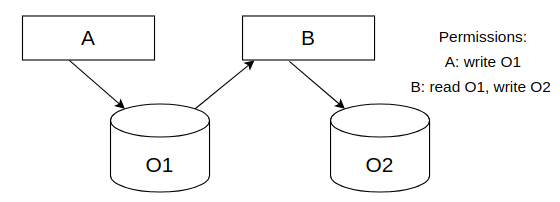
\includegraphics[width=0.90\textwidth]{resources/Chapter-1/cap1.png}
\centering
\end{figure}
This is what is called a Cross Application Poisoning attack. Taking this example into the ONOS environment and making it more specific we can say that application A writes to object O1 (having write permission on this object), application B reads the value of O1 and writes to object O2 the value of O1 (having read permissions on O1 and write on O2). In this case, if we imagine that application A is malicious, its goal is to write to object O2, but it has not been granted this permission and therefore cannot do it directly. However, it can do it indirectly by writing to O1, then the legitimate application A2 will write into O2 what the malicious application has decided.

In 2018 Ujcich et al. published the paper "Cross-App Poisoning in Software-Defined Networking" in which for the first time the term "Cross Application Poisoning" was invented. They designed a defense mechanism too that will be studied and discussed in the next section. The main problem with Role Based Access Control is that those policies don't have control over the usage of data and so how data is used after authorization. In their work they also present a working Cross Application Poisoning attack present in ONOS default applications (they used ONOS version 1.8.0, but it has been reproduced also in the latest ONOS version at the time of writing which is 2.7.0) \cite{cap-sdn}:
\begin{quoting}[font=itshape, begintext={"}, endtext={"}]
Consider the scenario in which an SDN controller provides host and flow rule services among its core functionalities. Suppose an adversary has compromised a host-tracking app that, as part of the app’s normal functionality, has permission to write to the host data store, but does not have permission to write flow rules. A second app performing routing has permission to read the host store and also to read and write flow rules. As part of its functionality, the routing app ensures that all hosts can be routed correctly, and it modifies flow rules as needed. Now suppose that the adversary modifies a host location in the host data store to point to a host that it has compromised. The routing app detects this change and rewrites flow rules to reflect the new location. Without being granted permission, the host-tracking app in this example has succeeded in effectively bypassing the RBAC-based system by having the routing app modify the network’s flow rules on the host-tracking app’s behalf.
\end{quoting}
Figure 1.5 shows a graphical representation of this attack scenario. This CAP attack example will be used as main reference for tests in the next sections. Implementations details for this attack and for a similar one (same concept but achieving different goals) will be provided in Section 2.2 (CAP attacks implementation).

\begin{figure}[t]
\caption{Malicious Host Tracking CAP attack}
\label{fig:cap2}
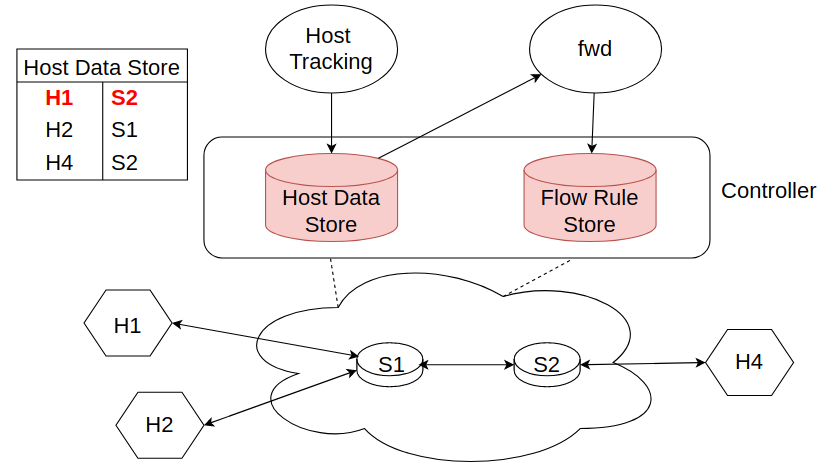
\includegraphics[width=1.0\textwidth]{resources/Chapter-1/cap2.png}
\centering
\end{figure}

We are going to see the formal definition of a Cross Application Poisoning attack, it's a simplified version of the one provided by Ujcich et al. in their paper. 

Consider:
\begin{itemize}
  \item A set of apps, denoted by A = \{a1, a2, ..., an\}
  \item A set of objects, denoted by O = \{o1, o2, ..., on\}
  \item A set of application read permissions, denoted by PR, that make it possible to access or read from objects.
  \item A set of application write permissions, denoted by PW, that make it possible to write, modify, or delete objects.
\end{itemize}

We then build a bipartite graph having as node classes the applications and the objects with their respective identifiers. The edges will then be added like this: if an application can write into an object, there will be an edge going from the application to the object; if instead an object can be read from an application the direction of the edge will be the opposite. As result we end up with a graph showing the read and write permissions between applications and shared objects. We call this graph the "CAP attack vector graph", and we define a CAP "vector" a chain of permissions that potentially can be exploited to carry out a CAP attack. Figure 1.6 shows the result graph: in the upper part we have three applications (a1, a2 and a3), while in the lower three objects (o1, o2 and o3). All the edges have the label "pX" where X is a number ranging from 1 to 7 because we have seven permissions in our policy example (we assume that the least privilege principle is applied and only the minimum set of permissions is granted). If we take as example the permission edge p1, this means that the application a1 is allowed to write (calling the proper APIs) into object o1. 

We can then define a CAP attack vector a path (remember that this is a bipartite graph and the edges direction will be alternated e.g. a1, o1, a2, o2,...) in the graph with these conditions:
\begin{itemize}
  \item starting with an application aX (aX being any application)
  \item has length greater or equal than 3
  \item has odd length (ends with an object)
\end{itemize}

\begin{figure}[h]
\caption{CAP attack vectors}
\label{fig:cap-vectors}
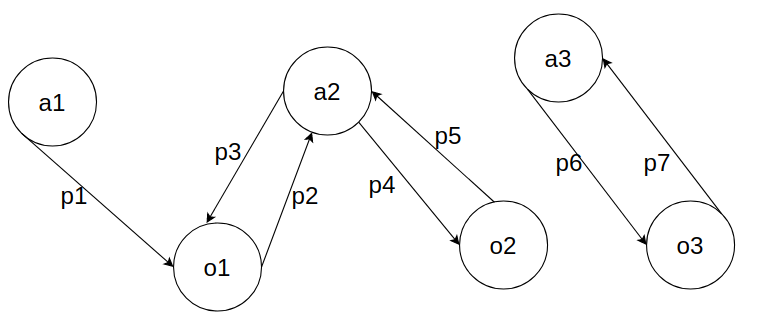
\includegraphics[width=1.0\textwidth]{resources/Chapter-1/cap-vectors.png}
\centering
\end{figure}

We formally define a CAP attack vector C on the graph g:
\begin{align}
C(g) = \{a1,o1,a2,o2,\;...,\;an,on\} \;|\; n >= 2; 
\end{align}

where n is odd.

In the Cross App Poisoning attack vector graph shown in Figure 1.6 there is only one potentially exploitable path that is $C1(g) = \{a1, o1, a2, o2\}$ using the permissions p1, p2, p4. 

It's crucial to notice two things: (a) it makes sense to build and talk about the CAP attack vector graph only if Security-Mode ONOS is active and the least privilege principle is applied, otherwise the graph would be a complete graph and every path can be an attack vector. (b) not all the CAP attack vectors can be exploited to carry out a working CAP attack: it could be that a data source in the chain is not directly influencing the next write resulting in a unexploitable CAP attack.

Regarding the point (b) there are some examples of failed attempts in Section 4.2 (Vulnerability research). 

\clearpage

\section{Existing solutions}
%% - why defense mechanisms in previous section don't help
In subsection 1.2 (Introduction to CAP attacks) we went through some security mechanisms provided by ONOS like Security-Mode ONOS. We saw also that this mode can help with the security posture of the whole architecture reducing the attack surface exposed to malicious applications. We've also understood that some actions can improve the overall security of the system, even though they are not provided by ONOS (like application and policy file signing). However, unfortunately, these methods are ineffective when it comes to Cross Application Poisoning attacks. We can see this attack methodology as a Security-Mode bypass or an effective way to mislead the security systems and make sure attackers don't get caught.

Other security mechanisms could be implemented to improve the overall system security, but those won't be effective too. For example, any mechanism implementing Role-Based Access Control can be bypassed by these attacks (exactly like Security-Mode ONOS) \cite{secmode}. Data shared using ONOS APIs can be kept confidential using TLS or any other cryptographically secure system, but this won't stop CAP attacks \cite{tlsapis}. Also signing all the trusted applications is not an effective security mechanism for CAP attacks: imagine we have a signed application from a trusted party. Even API abuse prevention is not deemed to be effective against CAP attacks \cite{aegis,dac}. This means we trust the developers and the entity and processes that created the application. So we can assume they didn't implement a CAP attack in that application. But applications can expose data and endpoints in the network (private but even public), this means an attacker could have a way to first of all attack the trusted application, then perform a CAP attack. This induces a false sense of security because we trust the entity that developed the application. Certain SDN controllers implement application sandboxing to prevent applications to use resources that should not be accessed by them (like file system does in operating systems) and this seems to be an effective mechanism; the problem is the concept itself of Cross Application Poisoning attack: a malicious application could induce a legitimate application to perform forbidden action on the first one's behalf \cite{rosemary}.

\medskip
We're going to see some defense mechanisms explained in the literature, how they work and what are their limitations.


\subsection{ProvSDN}

As shown in table regarding security issues in ONOS, the only security mechanisms available for Cross Application Poisoning attacks is ProvSDN. This is a model described in the paper "Cross-App Poisoning in Software-Defined Networking" by Ujcich et al. The authors started analyzing the CAP gadgets exploitable in ONOS default applications using Java abstract syntax trees. An abstract syntax tree is a (tree-based) structured representation of the source code of a program, in this case ONOS apps. They used javaparser to achieve the results, but other products are available for different programming languages. They analyzed all the available applications: 63 excluding the test one (using ONOS version 1.8.0). After this step the authors used field-sensitive interprocedural data flow
analysis to determine the sources and sinks useful to carry out CAP attacks. A "source" is defined as an ONOS API read call, while a "sink" is a ONOS API write call. The table below shows some of the results achieved using this method. The first field is the application vulnerable to CAP attack, the second and the third ones are respectively the source and the sink of the CAP gadget. This means every application having the source write permission can carry out a Cross Application Poisoning attack. As example, an application having the permission APP\_WRITE can poison the application openstacknetworking to achieve the permission FLOWRULE\_WRITE (e.g. attacker modifies the app ID to remove all flows with a given app ID). 

\begin{table}[h]
\begin{tabular}{lllll}
\hline
\thead{App} & \thead{Source} & \thead{Sink} & \thead{Attacker’s capabilities if \\source data have been\\ compromised by attacker} & \\ \cline{1-4}
\hline

\multicolumn{1}{l}{openstacknetworking} & \multicolumn{1}{l}{APP\_READ} & \multicolumn{1}{l}{FLOWRULE\_WRITE} & \makecell[l]{Attacker modifies the app ID\\to remove all flows with a\\given app ID} \\ \cline{1-4}

\multicolumn{1}{l}{openstacknode} & \multicolumn{1}{l}{APP\_READ} & \multicolumn{1}{l}{CLUSTER\_WRITE} & \makecell[l]{Attacker modifies the app ID\\to make an app run for \\leader election in a different\\ONOS topic} \\ \cline{1-4}

\multicolumn{1}{l}{openstacknode} & \multicolumn{1}{l}{APP\_READ} & \multicolumn{1}{l}{GROUP\_WRITE} & \makecell[l]{Attacker modifies the app ID\\to associate an app with a \\particular group handler} \\ \cline{1-4}

\multicolumn{1}{l}{routing} & \multicolumn{1}{l}{APP\_READ} & \multicolumn{1}{l}{CONFIG\_WRITE} & \makecell[l]{Attacker modifies the app ID\\to misapply a BGP configuration} \\ \cline{1-4}

\multicolumn{1}{l}{vtn} & \multicolumn{1}{l}{DEVICE\_READ} & \multicolumn{1}{l}{DRIVER\_WRITE} & \makecell[l]{Attacker misconfigures driver\\setup for a device (i.e., switch)} \\ \cline{1-4}

\multicolumn{1}{l}{vtn} & \multicolumn{1}{l}{HOST\_READ} & \multicolumn{1}{l}{FLOWRULE\_WRITE} & \makecell[l]{Attacker misconfigures flow rules\\based on a host with a particular\\MAC address} \\ \cline{1-4}

\multicolumn{1}{l}{fwd} & \multicolumn{1}{l}{PACKET\_READ} & \multicolumn{1}{l}{FLOWRULE\_WRITE} & \makecell[l]{Attacker injects or modifies an\\incoming packet to poison \\a flow rule} \\ \cline{1-4}

\end{tabular}
\end{table}

%% - spiegazione alto livello provsdn
ProvSDN leverages the concept of information flow: tracking how the data is used after authentication can block or detect Cross Application Poisoning attacks. The authors used a floating label model (based on Myers and Liskov’s Information Flow Control model) to define such approach. The Information flow control policy model is denoted by $I = (A,T, L,Ch, Re)$ and consists of:
\begin{itemize}
    \item\texttt{A set of apps}, denoted by A = \{a1, a2, . . . , ax\}.
    \item\texttt{A set of integrity tags}, denoted by $T = \{\tau1, \tau2, . . . , \tau t\}$.
    \item\texttt{Integrity labels that map apps to a subset of integrity tags}, denoted by $L : A -> P(T)$, where $P(T)$ is the power set of $T$.
    \item\texttt{An enforcement check policy on when to check for violations}, denoted by $Ch \in \{READS, WRITES\}$.
    \item\texttt{A response to perform when information flow is violated}, denoted by $Re \in \\\{BLOCK, WARN, NONE\}$.
\end{itemize}

Then the authors give these two definitions:
\begin{itemize}
    \item An application's integrity is defined relatively to another one: if the integrity tags set is a superset of the second one, the first application has higher integrity.
    \item The integrity of an object is defined as the same of the application having the lowest integrity label that contributed to its creation.
\end{itemize}

The authors defines "app" as both applications and switches, while the "objects" are the data stores and all the entities in the shared controller that can help delivering a Cross Application Poisoning attack. 

From the authors's definition, 
\begin{quoting}[font=itshape, begintext={"}, endtext={"}]
ProvSDN hooks all of the controller’s API interfaces to collect provenance from apps, builds a provenance graph, and serves as an online reference monitor by checking API requests against the IFC policy I. This allows us to prevent both known and unknown CAP attacks based on policy.
\end{quoting}


Here the term "data provenance" means tracking the data in order to understand how the system use those elements of information. The W3C PROV data model is used, which defines a directed acyclic graph to understand how data is used by actors in the system.

\begin{figure}[h]
\caption{ProvSDN (Cross-App Poisoning in Software-Defined Networking)}
\label{fig:provsdn}
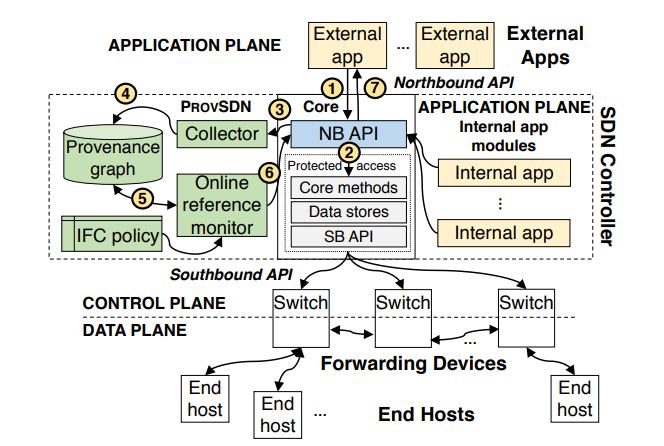
\includegraphics[width=1\textwidth]{resources/Chapter-1/provsdn.png}
\centering
\end{figure}

The figure 1.7 shows how ProvSDN works at high-level:
\begin{enumerate}
    \item An app makes a NB API request. 
    \item The NB API tentatively retrieves or inserts data related to the request.
    \item The collector processes the call information.
    \item The collector writes the provenance data to the provenance graph.
    \item The online reference monitor checks the provenance graph for violations according to the IFC policy.
    \item The IFC policy’s response is returned to the NB API.
    \item Depending on the response, the data may be returned to the app or may be written to the shared SDN control plane state.
\end{enumerate}


Depending on the policy definition, the behavior is different: (a) if the response is BLOCK, the action will be blocked or an alert will be triggered if action is WARN. (b) if the check policy is WRITES, the checks will be performed and blocked on writes, on reads instead if READS is specified. Integrity labels play a fundamental role here, for example if an application tries to read data generated from another one and the second has lower integrity with respect to the first one, the action will be blocked.

\medskip

The tests performed by the authors show that this approach works well and effectively blocks or detects Cross Application Poisoning attacks. However, even if there are some pros the are also drawbacks (explained by authors too). The main problem is the data-integrity label approach: if a low-integrity application writes on many objects, all those objects cannot be read by applications having an higher integrity label. This is a limiting constraint as the system cannot behave correctly, it's common that security mechanism limit in certain ways the functionalities, but in this case the system could occur in degradation of important operations. Another problem is the overall performance, from the tests performed by the authors ProvSDN seems to increase the ONOS controller packet handling by a factor of 2x on average, which is a considerable time addition in certain types of network. The authors suggest to use this method only \begin{quoting}[font=itshape, begintext={"}, endtext={"}]on the relatively infrequent control plane state changes rather than on each individual packet of a flow\end{quoting} This means that a Cross Application Poisoning attack could remain unnoticed if a frequent control plane state change is used. 

\subsection{vIFC}

The paper "Protecting Virtual Programmable Switches from Cross-App Poisoning (CAP) Attacks" by Lamb et al. highlights some ProvSDN limitations and defines a model that tries to address those issues. This new solution is called vIFC with the v standing for virtual, we are going to see the limitations found by the authors.\cite{virtual-cap-sdn}

The first limitation arises when the network uses virtual programmable switches. In such scenario a switch is a software deployed in a physical device and this implies some actions that were
\begin{wrapfigure}[17]{h}{0.55\textwidth}
\caption{CAP with virtual switches interactions}
\label{fig:vcap}
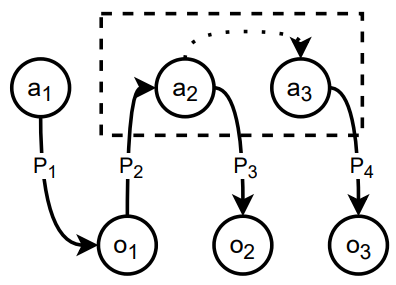
\includegraphics[width=0.55\textwidth]{resources/Chapter-1/v-cap.png}
\end{wrapfigure}
not considered in the study that created ProvSDN. 
There are multiple ways to implement virtual switches, one method is to virtualize multiple virtual switch images in a single device through P4 language (Hyper4 being one of the most famous example); another technique uses switch program composition (P4Visor being on the most famous example) merging the code of different switches in a single program; another solution, like P4VBox, divide the available resources and assign them to virtual switches. 

Figure 1.8 graphically shows what a Cross Application Poisoning attack could look like when programmable virtual switches are used. There are three applications used (as in the previous paper both ONOS applications and switches are considered apps) named a1, a2, a3 and three objects named o1, o2, o3. a1 starts the interaction writing something to the object o1, then the application a2 reads from the object o1. Here there is an "anomaly" not taken into consideration in the previous paper: a2 being virtualized in the same environment of a3 can communicate with a3 directly without using the ONOS APIs. Finally a3 writes into the object o3. All the interactions are legitimate since the applications use regular ONOS permissions to access APIs and the internal communication between virtualized switches. ProvSDN cannot detect such Cross Application Poisoning attacks because the internal communication is not tracked by the provenance graph, so it will see only the paths a1-o1-a2 and a3-o3 in which there is not present a CAP attack.
\begin{figure}[h]
\caption{CAP attack leveraging virtual switches}
\label{fig:vifc}
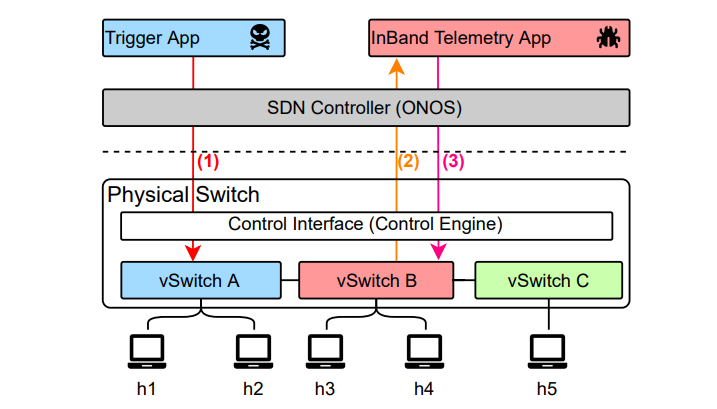
\includegraphics[width=1.0\textwidth]{resources/Chapter-1/vIFC.png}
\centering
\end{figure}
Figure 1.9 describes an example of CAP attack provided in the paper. In this scenario two ONOS applications are used: the InBand Telemetry (INT) App and the Trigger one. The INT application receives statistical data from the network and moves network packets away from busiest switches to avoid overloading; instead the Trigger application is the malicious one. As the figure shows there is only one physical switch which virtualizes three switches (vSwitch A, B and C) connected to five hosts. The switches are monitored using Multi-Hop Route Inspection, doing so it's possible to track switches' queue occupancy. The INT application reroutes traffic when the queue occupancy is above a certain threshold. The Cross Application Poisoning attack works in this way:
\begin{enumerate}
    \item The Trigger application sends a fake telemetry data packet which says that the queue occupancy is above the safety threshold.
    \item The packet sent in point 1 is crafted in a way that an out-of-band flow is needed and vSwitchA sends the packet to vSwitchB using an internal connection inside the physical switch. 
    \item The packet is then sent to the INT application which, as part of its main functions, reroutes networks traffic from the busiest switches to quiet ones. 
\end{enumerate}

This type of interaction can be replicated many times resulting in network congestion and denial of service. This is a simple example but the authors provided another example with 7 steps using FPGA switches achieving the same results.
\medskip

Another problem found by the authors is the use of multiple controllers. They provide another example of Cross Application Poisoning attack leveraging programmable virtual switches and multiple controllers. Consider a scenario in which we have three applications and two controllers. The first application is malicious, while the second and the third one are legitimate. The first and the second application use the first controller, while the third one uses the second controller. In the data-plane there is a single physical switch hosting three virtualized switches. We can then have two types of Cross Application Poisoning attacks: (a) the first one is exactly the same as the previous example, using the malicious application instead of the Trigger app and the second legitimate application taking the role of the INT application. (b) The second attack is carried out crafting a packet that requires using an out-of-band communication between vSwitchA and vSwitchC. Since they use a different controller ProvSDN cannot effectively detect that type of interaction and so the attack remains unnoticed.
\medskip

\begin{wrapfigure}[17]{h}{0.55\textwidth}
\caption{vIFC architecture}
\label{fig:vcap}
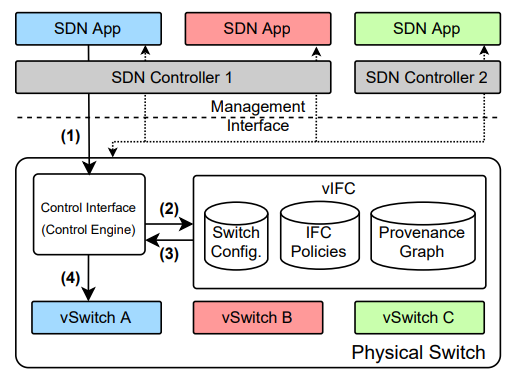
\includegraphics[width=0.55\textwidth]{resources/Chapter-1/vifc-arch.png}
\end{wrapfigure}

%% vIFC implementation
The solution to these problems was named by the author "vIFC" or virtual switch information flow control. It's clear as also the authors state that it's an adaptation of ProvSDN to address the issues explained above. A change made in vIFC was to move the collection and detection engine at the control-data interface (in ProvSDN was in the control plane). Doing so it's possible to control the interactions between the controller and virtual switches. In ProvSDN this was not possible since at controller level it's only possible to have a view of the single physical switch. Putting the checks at a lower level mitigates also the problem of multiple controllers, in this case even if two or more controllers are used it's possible to get a provenance graph including CAP attacks this particular environment setup. The elements of the detection model are more or less the same of ProvSDN: a control engine where all the checks are implemented, an IFC policy database where all the policies regarding the allowed flows are stored, a provenance graph and the only additional element is the switch configuration repository (Where the switches configuration are stored). The detection check works as the same as ProvSDN: an application calls an API (like in ProvSDN the checks could be enforced at read or write access), the control engine gathers all the necessary information to understand if the API is allowed or not and adds the entry to the provenance graph to understand if there is a path violating at least one of the IFC policies. If everything is okay the access is allowed, otherwise it's blocked. As the authors state, it's easy to get information about communications between apps and switches, but it's difficult to understand when two switches are communicating using out-of-band channels. To get this information the authors implemented a packet comparison solution in which they compare packets metadata coming from virtualized switches. At every check performed by the control engine not only the interactions between apps and switches are considered, but also the out-of-band communications between virtualized switches.

We saw that vIFC it's not a brand new solution, but it's complementary to ProvSDN and exactly like ProvSDN it has some limitations and drawbacks. One limitation is the performance overhead brought by the runtime checks performed by the control engine (same as ProvSDN). In high performance networks these latency values added by vIFC checks could be very problematic: on average vIFC is ten times slower than the baseline. Moreover, the authors state that another problem could arise when virtual switches are overloaded and vIFC could not behave correctly and so Cross Application Poisoning attacks could remain unnoticed.

\subsection{Changing point of view} 

All the existing solutions providing security mechanisms to Cross Application Poisoning attacks are explained in the previous sections. One is ProvSDN and the second is called vIFC that is an adaptation of the first one with additional defense mechanisms for particular environments. Both solutions use an information flow graph with the aim of tracking data after authorization. The main idea is to understand how data is used by applications authorized to perform restricted API calls. We saw that Cross Application Poisoning attacks can be well represented by paths with spacial characteristics using a bipartite graph composed by applications and data objects (mainly data stores). Even if these solutions provide a model to prevent or detect (depending on administrator's choice) CAP attacks there are some important limitations and problems:

%% - see previous solutions limitations
%% - source code
\begin{itemize}
    \item The integrity labels model used by ProvSDN (even if it makes sense from a security point of view) limits by a lot the network capabilities. As stated from the authors there could be legitimate API calls blocked by this model. 
    \item Moreover, worse, low integrity malicious applications can exploit their status writing on all the objects they have access to. Doing so, all the applications having an integrity status higher than the malicious one won't be able to access the poisoned objects. This is just another way to perform a poisoning attack.
    \item Both solutions dramatically increase network performance overhead, which in certain cases could be crucial. 
    \item In order to build the Information Flow Policy, we need to know which permissions an application need in order to access the required ONOS APIs. With open source applications this is simple (even though there's no need to entirely understand what the application is doing), we just need to search for exposed ONOS APIs in the source code. What about closed source applications? It could even be that we have only the binary (ONOS Java compiled archive, a .oar file) ready to be installed in ONOS environment. If we have to follow the least privilege principle to build the permission graph this is not possible without the permissions needed by applications. Ignoring the permissions graph and using a complete graph (each application have access to all the APIs) can end up in two situations (a) vast majority of API calls are blocked or (b) any application can access all APIs directly and so there is no need to talk about Cross Application Poisoning attack (e.g. if a malicious application wants to install a new flow rule, it just needs to call the proper API).
\end{itemize}

Once listed the limitations of the available solutions, there are some aspects of Software Defined Networks and Cross Application Poisoning attacks that need to be pointed out. First of all installing a new application it's not something very common. Deciding to use a new program in a network is something that should be done very carefully and it's not a matter of seconds: it's a choice that should be analyzed in order to understand which problems could arise with a new network configuration. As example of bad configurations, see the paper "Digital Twin Manager: A Novel Framework to
Handle Conflicting Network Applications" in which the authors provide example of SDN environment where the installed applications have conflicting goals, which results in performance degradation \cite{dt-manager}. It would be better to have a solution in which it doesn't matter if the administrator has access to source code or the permissions list needed for an application to run correctly; even if only the compiled binary is provided, it should be possible to test the environment for Cross Application Poisoning attacks. Since network performance is a critical characteristic, a solution that doesn't affect or has a minimal overhead over traffic latency would be better.
\medskip

To address all these elements, in following sections a new solution is provided. The main idea is to test applications offline rather than online: the security tests are performed only when the administrator decides to install a new application into an existing environment. The tests are performed into an exact copy of the production environment. This solves the problem of performance overhead (as it doesn't have overhead at all), the applications that don't provide the required permissions list can still be tested (even if only a compiled binary is provided) and the capabilities limitation (as it doesn't use any integrity label model).

\clearpage